
\documentclass[12pt]{article}
 
\usepackage[margin=1in]{geometry}
\usepackage{amsmath,amsthm,amssymb}
\usepackage{slashed}
\usepackage{bbold}
\usepackage{graphicx}
 
\newcommand{\N}{\mathbb{N}}
\newcommand{\Z}{\mathbb{Z}}
 
\newenvironment{question}[2][Question]{\begin{trivlist}
\item[\hskip \labelsep {\bfseries #1}\hskip \labelsep {\bfseries #2.}]}{\end{trivlist}}
\newenvironment{questionpart}[2][Part]{\begin{trivlist}
\item[\hskip \labelsep \hskip \labelsep {\bfseries (#2)}]}{\end{trivlist}}

\newenvironment{solution}{\begin{proof}[Solution]}{\end{proof}}
 
\begin{document}
 
% --------------------------------------------------------------
%                         Start here
% --------------------------------------------------------------
 
\title{QFT HW 13}%replace X with the appropriate number
\author{Lucas Nestor}
 
\maketitle
 
\begin{question}{13.3}

\end{question}

\begin{questionpart}{a}
Evaluate the phase space integrals for $1\rightarrow 2$ decays. Show to total rate is
\begin{equation*}
    \Gamma(\phi\rightarrow e^++e^-)=\frac{\sqrt{1-4x^2}}{8\pi m^\phi}|\mathcal{M}|^2 \qquad x=\frac{m_e}{m_\phi}
\end{equation*}
\end{questionpart}
 
\begin{solution}

First we want to evaluate the phase space integral. We will assume that $|\mathcal{M}|^2$ is independent of $\vec{p}_2$ and $\vec{p}_3$.
\begin{equation*}
    \int\frac{d^3p_2}{(2\pi)^3}\frac{1}{2E_2}\frac{d^3p_3}{(2\pi)^3}\frac{1}{2E_3}(2\pi)^4\delta^4(p_1-p_2-p_3)
\end{equation*}

First, obviously we can take some factors out of the integral to make things easier. We will also split up the delta function into a time part and space part.
\begin{equation*}
    \frac{1}{16\pi^2}\int d^3p_2 d^3p_3 \frac{1}{E_2 E_3}\delta(E_1-E_2-E_3)\delta^3(\vec{p}_1-\vec{p}_2-\vec{p}_3)
\end{equation*}

We will work in the rest frame of the decaying particle, so $E_1=m_1$ and $\vec{p}_1=\vec{0}$.
\begin{equation*}
    \frac{1}{16\pi^2}\int d^3p_2 d^3p_3 \frac{1}{E_2 E_3}\delta(m-E_2-E_3)\delta^3(\vec{p}_2+\vec{p}_3)
\end{equation*}

Now we perform the integral over $d^3p_3$, which gives us $\vec{p}_3=-\vec{p}_2$. This means that $E_2=\sqrt{p_2^2+m_2^2}$ and $E_3=\sqrt{p_2^2+m_3^2}$.
\begin{equation*}
    \frac{1}{16\pi^2}\int d^3p_2 \frac{1}{E_2 E_3}\delta(m_1-E_2-E_3)
\end{equation*}

It would be nice get rid of that $\delta$-function now and set $E_2+E_3=m_1$. However, we are integrating over $d^3p_2$, so we have to massage either our $\delta$-function or integration range to match each other. I will choose the latter. We will switch to spherical coordinates first.
\begin{equation*}
    \frac{1}{16\pi^2}\int p_2^2dp_2d\Omega_2 \frac{1}{E_2 E_3}\delta(m_1-E_2-E_3)
\end{equation*}

Now we want to make a substitution for $E_1+E_2$.
\begin{equation*}
    d(E_2+E_3)=dE_2+dE_3=d\left(\sqrt{p_2^2+m_2^2}\right)+d\left(\sqrt{p_2^2+m_3^2}\right)=\frac{p_2dp_2}{E_2}+\frac{p_2dp_2}{E_3}
\end{equation*}

We can rearrange this to give us what we need.
\begin{equation*}
    \frac{d(E_2+E_3)}{E_2+E3}=\frac{p_2}{E_2E_3}dp_2
\end{equation*}

This fits nicely with what we already had, so we can plug it in.
\begin{equation*}
    \frac{1}{16\pi^2}\int p_2 d(E_2+E_3)d\Omega_2\frac{1}{E_2+E_3}\delta(m_1-E_2-E_3)
\end{equation*}

We can now evaluate this integral to get something simple. We also can evaluate the integral over $\Omega_2$, noting that it is just $4\pi$ since we have no dependence on $\phi$ or $\theta$.
\begin{equation*}
    \frac{1}{4\pi}\frac{p_2}{m_1}
\end{equation*}

Now let's plug back into the equation for $\Gamma$. Again, $E_1=m_1$ since we are in the rest frame of the decaying particle.
\begin{equation*}
    \Gamma(1\rightarrow 2)=\frac{p_2}{8\pi m_1^2}|\mathcal{M}|^2
\end{equation*}

In the case of $\phi\rightarrow e^++e^-$, $E_2=E_3=\frac{m_1}{2}$ due to the delta function.
\begin{equation*}
    p_2=\sqrt{E_2^2-m_2^2}=E_2^2\sqrt{1-\frac{m_2^2}{E_2^2}}=\frac{m_2}{2}\sqrt{1-\frac{4m_2^2}{m_1^2}}
\end{equation*}

Now we arrive at our solution that was desired.
\begin{equation*}
    \Gamma(\phi\rightarrow e^+e^-)=\frac{\sqrt{1-4x^2}}{8\pi m_\phi}|\mathcal{M}|^2 \qquad x=\frac{m_e}{m_\phi}
\end{equation*}
\end{solution}

\begin{questionpart}{b}
Evaluate $\Gamma$ (summed over final spins and averaged over initial spins if necessary) for the following cases:
\begin{enumerate}
    \item $\phi$ is a scalar with interaction $g_S \phi \overline{\psi}\psi$ 
    \item $\phi$ is a pseudoscalar with interaction $ig_P \phi \overline{\psi}\gamma_5\psi$ 
    \item $\phi$ is a vector with interaction $g_V \phi_\mu \overline{\psi}\gamma^\mu\psi$ 
    \item $\phi$ is an axial vector with interaction $ig_A \phi_\mu \overline{\psi}\gamma^\mu\gamma_5\psi$ 
\end{enumerate}
\hfill \break
Give the intermediate steps:
\begin{itemize}
    \item Express $\mathcal{M}$ in terms of a spinor product.
    \item Express $\sum_{\text{spins}}|\mathcal{M}|^2$ in terms of a Dirac trace
    \item Express $\sum_{\text{spins}}|\mathcal{M}|^2$ in terms of masses
\end{itemize}
\end{questionpart}

\begin{solution}
We are seeking a decay of particle $\phi$ into $e^+$ and $e^-$. We don't need any propagators because there are no internal lines. The vertex rules are simply our interactions multiplied by $-i$. Each diagram has two outgoing spinors, so we will get a $\overline{u}$ and $v$ spinor.
\begin{align*}
    g_S\phi\overline{\psi}\psi &\rightarrow -i g_S \\
    ig_P\phi\overline{\psi}\gamma_5\psi &\rightarrow g_P \gamma_5 \\
    g_V \phi_\mu \overline{\psi}\gamma^\mu\psi &\rightarrow -ig_V\gamma^\mu \\
    ig_A\phi_\mu\overline{\psi}\gamma^\mu\gamma_5\psi &\rightarrow g_A \gamma^\mu \gamma_5
\end{align*}

Now we can calculate $i\mathcal{M}$. I will start with the first case.
\newline

\textbf{Scalar}

The matrix element is given by:
\begin{equation*}
    i\mathcal{M}=(-ig_S)\overline{u}(p_2)v(p_3)
\end{equation*}

Now we sum over spins.
\begin{align*}
    \sum_{\text{spins}} |\mathcal{M}|^2&=g_S^2\sum_{\text{spins}}\overline{u}(p_2)v(p_3)\overline{v}(p_3)u(p_2) \\
    &= g_S^2\text{Tr}[(\slashed{p}_2+m)(\slashed{p}_3-m)]
\end{align*}

Now we can evaluate this trace.
\begin{align*}
    \text{Tr}[(\slashed{p}_2+m)(\slashed{p}_3-m)]&=p_2^\mu p_3^\nu\text{Tr}[ (\gamma_\mu \gamma_\nu)]-m p_2^\mu\text{Tr}[ (\gamma_\mu)]+m p_3^\mu\text{Tr}[ (\gamma_\mu)]-m^2\text{Tr}[\mathbb{1}] \\
    &= p_2^\mu p_3^\nu 4g_{\mu\nu} - 0 + 0 - 4m^2 \\
    &= 4(p_2^\mu p_{3\mu}-m^2)
\end{align*}

We want to express $p_2^\mu p_{3\mu}$ in terms of the masses. We can do this using 4-momentum conservation.
\begin{align*}
    p_1^\mu=p_2^\mu+p_3^\mu \rightarrow (p_1)^2=(p_2)^2+(p_3)^2+2p_2\cdot p_3 \rightarrow p_2 \cdot p_3 =\frac{1}{2}m_\phi^2-m_e^2
\end{align*}

So our trace is:
\begin{align*}
    \text{Tr}[\cdots]=4(\frac{1}{2}m_\phi^2-m_e^2-m_e^2)=2(m_\phi^2-4m_e^2)=2m_\phi^2(1-4x^2)
\end{align*}

Which makes our sum of spins:
\begin{align*}
    \sum_{\text{spins}} |\mathcal{M}|^2&=2g_S^2m_\phi^2(1-4x^2)
\end{align*}

Now we plug that in to our equation for $\Gamma$.
\begin{align*}
    \Gamma(\phi_S\rightarrow e^+e^-)&=\frac{m_\phi g_S^2}{4\pi}(1-4x^2)^\frac{3}{2}
\end{align*}

\textbf{Pseudoscalar}

Now we can look at the pseudoscalar part.
\begin{align*}
    i\mathcal{M}=g_P\overline{u}(p_2)\gamma_5v(p_3)
\end{align*}

We need to be careful when squaring $\mathcal{M}$ now because of the $\gamma_5$. It turns out that we pick up a negative sign when swapping the $\gamma_5$ and $\gamma_0$.
\begin{align*}
    |\mathcal{M}|^2&=\mathcal{M}\mathcal{M}^\dagger=g_p^2 \overline{u}(p_2)\gamma_5 v(p_3) v^\dagger(p_3)\gamma_5 \gamma_0 u(p_2) \\
    &=-g_P^2\overline{u}(p_2)\gamma_5v(p_3)\overline{v}(p_3)\gamma_5u(p_2)
\end{align*}

And summing over spins. We should be careful to keep track of indices.
\begin{align*}
    \sum_{\text{spins}} |\mathcal{M}|^2&=-g_P^2\sum_{\text{spins}}\overline{u}(p_2)\gamma_5v(p_3)\overline{v}(p_3)\gamma_5u(p_2) \\
    &= -g_P^2\sum_{\text{spins}}\overline{u}(p_2)_a(\gamma_5)_{ab}v(p_3)_b \overline{v}(p_3)_c (\gamma_5)_{cd}u(p_2)_d
\end{align*}

Now we rearrange this to get something we can turn into a trace.
\begin{align*}
    \sum_{\text{spins}} |\mathcal{M}|^2&=-g_P^2\sum_{\text{spins}}u(p_2)_d\overline{u}(p_2)_av(p_3)_b \overline{v}(p_3)_c(\gamma_5)_{cd}u(p_2)_d(\gamma_5)_{ab} \\
    &= -g_P^2\text{Tr}[(\slashed{p_2}+m)\gamma_5 (\slashed{p_3}-m)\gamma_5]
\end{align*}

Now we can evaluate this trace, remembering that $\gamma_5^2=\mathbb{1}$ and $\{\gamma_5,\gamma_\mu\}=0$.
\begin{align*}
    \text{Tr}[(\slashed{p_2}+m)\gamma_5 (\slashed{p_3}-m)\gamma_5] &= p_2^\mu p_3^\nu \text{Tr}[\gamma_\mu \gamma_5 \gamma_\nu \gamma_5]-mp_2^\mu\text{Tr}[\gamma_\mu \gamma_5^2]+mp_3^\mu\text{Tr}[\gamma_5\gamma_\mu\gamma_5]-m^2\text{Tr}[\gamma_5^2] \\
    &= -4 p_2^\mu p_{3\mu}-0+0-4m^2 \\
    &= -4(p_2^\mu p_{3\mu}+m^2) = -2m_\phi^2
\end{align*}

Thus, our sum of spins is:
\begin{align*}
    \sum_{\text{spins}} |\mathcal{M}|^2&=2g_P^2m_\phi^2
\end{align*}

And plugging this into $\Gamma$:
\begin{align*}
    \Gamma(\phi_P\rightarrow e^+e^-)=\frac{m_\phi g_P^2}{4\pi}\sqrt{1-4x^2}
\end{align*}

\textbf{Vector}

Next, we move onto the vector case. Now we need to add in the polarization vector of the incoming particle. 
\begin{align*}
    i\mathcal{M}=-ig_V\overline{u}(p_2)\gamma_\mu v(p_3) \epsilon^\mu
\end{align*}

The procedure is the same as before. However, now we need to average of initial spins in addition to sum over final spins. Since this is a spin-1 particle, we will sum over the 3 spin states and divide by 3.
\begin{align*}
    \overline{\sum}|\mathcal{M}^2|&=\frac{1}{3}g_V^2\sum_i\epsilon_i^\mu \epsilon_i^{*\nu} \sum_\text{spins}\overline{u}(p_2)\gamma_\mu v(p_3)\overline{v}(p_3)\gamma_\nu u(p_2) \\
    &= \frac{1}{3}g_V^2\sum_i\epsilon_i^\mu \epsilon_i^{*\nu}\sum_{\text{spins}}\overline{u}(p_2)_a(\gamma_\mu)_{ab}v(p_3)_b \overline{v}(p_3)_c (\gamma_\nu)_{cd}u(p_2)_d \\
    &= \frac{1}{3}g_V^2\sum_i\epsilon_i^\mu \epsilon_i^{*\nu}\sum_{\text{spins}}u(p_2)_d\overline{u}(p_2)_av(p_3)_b \overline{v}(p_3)_c(\gamma_\mu)_{cd}u(p_2)_d(\gamma_\nu)_{ab} \\
    &= \frac{1}{3}g_V^2\sum_i\epsilon_i^\mu \epsilon_i^{*\nu}\text{Tr}[(\slashed{p_2}+m)\gamma_\nu (\slashed{p_3}-m)\gamma_\mu]
\end{align*}

To evaluate this trace, we note that any trace of an odd number of $\gamma_\mu$ matrices is $0$ and $\text{Tr}[\gamma_\rho \gamma_\nu \gamma_\sigma \gamma_\mu]=4(g_{\rho\nu} g_{\sigma \mu} + g_{\rho\mu} g_{\nu\sigma} - g_{\rho\sigma} g_{\nu\mu})$.
\begin{align*}
    \text{Tr}[\cdots]&=p_2^\rho p_3^\sigma \text{Tr}[\gamma_\rho \gamma_\nu \gamma_\sigma \gamma_\mu] - mp_2^\rho \text{Tr}[\gamma_\rho \gamma_\nu \gamma_\mu] + mp_3^\rho \text{Tr}[\gamma_\nu \gamma_\rho \gamma_\mu] -m^2 \text{Tr}[\gamma_\nu \gamma_\mu] \\
    &= 4 p_2^\rho p_3^\sigma(g_{\rho\nu} g_{\sigma \mu} + g_{\rho\mu} g_{\nu\sigma} - g_{\rho\sigma} g_{\nu\mu})-0+0-4m^2 g_{\nu\mu} \\
    &= 4(p_{2\nu} p_{3\mu} + p_{2\mu} p_{3\nu}-p_{2\rho}p_3^\rho g_{\mu\nu})-4m^2g_{\mu\nu} \\
    &= 4p_{2\nu} p_{3\mu} + 4p_{2\mu} p_{3\nu} - 4g_{\mu\nu}(\frac{1}{2}m_\phi^2 -m_e^2)-4m_e^2g_{\mu\nu} \\
    &= -2 g_{\mu\nu}m_\phi^2+4(p_{2\nu} p_{3\mu} + p_{2\mu} p_{3\nu})
\end{align*}

When contracted with our polarization vectors, we get this:
\begin{align*}
    \overline{\sum}|\mathcal{M}^2|&=\frac{1}{3}g_V^2 \sum_i\epsilon_i^\mu \epsilon_i^{*\nu} (-2g_{\mu\nu}m_\phi^2+4(p_{2\nu} p_{3\mu} + p_{2\mu} p_{3\nu})) \\
    &= \frac{2}{3}g_V^2\sum_i(4(\epsilon^i_\mu p_2^\mu)(\epsilon^{i*}_\nu p_3^\nu)-\epsilon^2 m_\phi^2)
\end{align*}

There are two things to note. First, $\epsilon_{i\mu}\epsilon_i^\mu=-1$ by our choice of normalization (this holds for each $i$, not summed over $i$). Thus, $\sum_i \epsilon_i^2=-3$. Next, we need to evaluate the $\epsilon_\mu p^\mu$ factors. To do this, we will use the basis for massive spin-1 polarization vectors found in Schwartz 8.30 and 8.31. These are given by $\epsilon_\mu^1=(0,1,0,0)$, $\epsilon_\mu^2=(0,0,1,0)$, and $\epsilon_\mu^3=(k_z/m,0,E/m)$. However, we will work in the rest frame of the decaying particle, so $\epsilon_\mu^3=(0,0,0,1)$. Now, without loss of generality, we will take the direction of decay to be the z-axis, so that $p_2^\mu=(E_2,0,0,p_{2z})$ and $p_3^\mu=(E_3,0,0,p_{3z})$. Using these expicit 4-vectors, we can continue our calculation.
\begin{align*}
    \sum_i(\epsilon_\mu^ip_2^\mu)(\epsilon_\mu^ip_3^\mu)=(-p_{2z})(-p_{3z})
\end{align*}

Note that only the $i=3$ term contributes because of our choice of momentum. From conservation of momentum, $p_{2z}=-p_{3z}$.
\begin{align*}
    \sum_i(\epsilon_\mu^ip_2^\mu)(\epsilon_\mu^ip_3^\mu)=-p_{2z}^2=m_e^2-E_2^2
\end{align*}

Lastly, conservation of energy tells us that $m_\phi=E_2+E_3$. But, like we said, $E_2=E_3$ in this frame, so $E_2=\frac{1}{2}m_\phi$.
\begin{align*}
    \sum_i(\epsilon_\mu^ip_2^\mu)(\epsilon_\mu^ip_3^\mu)=m_e^2-\frac{1}{4}m_\phi^2
\end{align*}

We can plug this into our sum of spins.
\begin{align*}
    \overline{\sum}|\mathcal{M}|^2&=\frac{2}{3}g_V^2(4m_e^2-m_\phi^2+3m_\phi^2) \\
    &=\frac{4}{3}g_V^2m_\phi^2(1+2x^2)
\end{align*}

Now we plut this into our decay rate.
\begin{align*}
    \Gamma(\phi_V\rightarrow e^+e^-)&=\frac{\sqrt{1-4x^2}}{8\pi m_\phi}\frac{4}{3}g_V^2m_\phi^2(1+x^2) \\
    &= \frac{g_V^2m_\phi}{6\pi}\sqrt{1-4x^2}(1+2x^2)
\end{align*}

\textbf{Axial Vector}

Our last task is to do the same analysis with the axial vector particle.
\begin{align*}
    i\mathcal{M}=-ig_A\overline{u}(p_2)\gamma_\mu \gamma_5 v(p_3) \epsilon^\mu
\end{align*}

Because we have $\gamma_5$ again, we need to be careful about signs. However, now we also have a $\gamma_\mu$. This means that we need to swap $\gamma_5$ twice, pikcing up 2 negative signs that cancel.We also will need to average over incoming spins.
\begin{align*}
    \overline{\sum}|\mathcal{M}^2|&=\frac{1}{3}g_A^2\sum_i\epsilon_i^\mu \epsilon_i^{*\nu}\sum_\text{spins}\overline{u}(p_2)\gamma_\mu \gamma_5 v(p_3)\overline{v}(p_3)\gamma_\nu \gamma_5 u(p_2) \\
    &= \frac{1}{3}g_V^2\sum_i\epsilon_i^\mu \epsilon_i^{*\nu}\sum_{\text{spins}}\overline{u}(p_2)_a(\gamma_\mu\gamma_5)_{ab} v(p_3)_b \overline{v}(p_3)_c (\gamma_\nu\gamma_5)_{cd}u(p_2)_d \\
    &= \frac{1}{3}g_V^2\sum_i\epsilon_i^\mu \epsilon_i^{*\nu}\sum_{\text{spins}}u(p_2)_d\overline{u}(p_2)_av(p_3)_b \overline{v}(p_3)_c(\gamma_\mu\gamma_5)_{cd}u(p_2)_d(\gamma_\nu\gamma_5)_{ab} \\
    &= \frac{1}{3}g_V^2\sum_i\epsilon_i^\mu \epsilon_i^{*\nu}\text{Tr}[(\slashed{p_2}+m)\gamma_\nu\gamma_5 (\slashed{p_3}-m)\gamma_\mu\gamma_5]
\end{align*}

We have all the tools needed to evaluate this trace.
\begin{align*}
    \text{Tr}[\cdots]&=p_2^\rho p_3^\sigma \text{Tr}[\gamma_\rho \gamma_\nu \gamma_5 \gamma_\sigma \gamma_\mu \gamma_5] + mp_2^\rho \text{Tr}[\gamma_\rho \gamma_\nu \gamma_\mu \gamma_5] + mp_3^\rho \text{Tr}[\gamma_\nu\gamma_5 \gamma_\rho \gamma_\mu\gamma_5] -m^2 \text{Tr}[\gamma_\nu \gamma_5\gamma_\mu\gamma_5] \\
    &=p_2^\rho p_3^\sigma \text{Tr}[\gamma_\rho \gamma_\nu\gamma_\sigma \gamma_\mu] + mp_2^\rho \text{Tr}[\gamma_\rho \gamma_\nu  \gamma_\mu ] - mp_3^\rho \text{Tr}[\gamma_\nu \gamma_\rho \gamma_\mu] +m^2 \text{Tr}[\gamma_\nu \gamma_\mu] \\
    &= 4 p_2^\rho p_3^\sigma(g_{\rho\nu} g_{\sigma \mu} + g_{\rho\mu} g_{\nu\sigma} - g_{\rho\sigma} g_{\nu\mu})-0+0+4m^2 g_{\nu\mu} \\
    &= 4(p_{2\nu} p_{3\mu} + p_{2\mu} p_{3\nu}-p_{2\rho}p_3^\rho g_{\mu\nu})-4m^2g_{\mu\nu} \\ 
    &= 4p_{2\nu} p_{3\mu} + 4p_{2\mu} p_{3\nu}-4g_{\mu\nu}(\frac{1}{2}m_\phi^2-m_e^2)+4m_e^2g_{\mu\nu} \\
    &= 2g_{\mu\nu}(4m_e^2-m_\phi^2)+4(p_{2\nu} p_{3\mu}+p_{2\mu}p_{3\nu})
\end{align*}

We already know how to contract this with the polarizations.
\begin{align*}
    \overline{\sum}|\mathcal{M}|^2&=\frac{1}{3}g_A^2 \sum_i\epsilon_i^\mu \epsilon_i^{*\nu}\left(2g_{\mu\nu}(4m_e^2-m_\phi^2)+4(p_{2\nu} p_{3\mu}+p_{2\mu}p_{3\nu})\right) \\
    &= \frac{2g_A^2}{3}\left((\sum_i\epsilon_i^2)(4m_e^2-m_\phi^2)+4(m_e^2-\frac{1}{4}m_\phi^2)\right) \\
    &= \frac{2g_A^2}{3}\left(-12m_e^2+3m_\phi^2+4m_e^2-m_\phi^2\right) \\
    &= \frac{2g_A^2}{3}(2m_\phi^2-8m_e^2)=\frac{4}{3}g_A^2m_\phi^2(1-4x^2)
\end{align*}

And we plug this into our decay rate.
\begin{align*}
    \Gamma(\phi_A\rightarrow e^+e^-)&=\frac{\sqrt{1-4x^2}}{8\pi m_\phi}\frac{4}{3}g_A^2m_\phi^2(1-4x^2) \\
    &= \frac{g_A^2m_\phi}{6\pi}(1-4x^2)^\frac{3}{2}
\end{align*}

\textbf{Summary}

I will summarize all the parts we had to do. First, the spinor products:
\begin{align*}
    i\mathcal{M}_S&=(-ig_S)\overline{u}(p_2)v(p_3) \\
    i\mathcal{M}_P&=(g_P)\overline{u}(p_2)\gamma_5v(p_3) \\
    i\mathcal{M}_V&=(-ig_V)\overline{u}(p_2)\gamma_\mu v(p_3)\epsilon^\mu \\
    i\mathcal{M}_A&=(g_A)\overline{u}(p_2)\gamma_\mu\gamma_5v(p_3)\epsilon^\mu
\end{align*}

Next, the traces.
\begin{align*}
    \sum_\text{spins}|\mathcal{M}_S|^2&=g_S^2\text{Tr}[(\slashed{p_2}+m) (\slashed{p_3}-m)] \\
    \sum_\text{spins}|\mathcal{M}_P|^2&=-g_P^2\text{Tr}[(\slashed{p_2}+m) \gamma_5(\slashed{p_3}-m)\gamma_5] \\
    \sum_\text{spins}|\mathcal{M}_V|^2&=\frac{1}{3}g_V^2\epsilon^\mu\epsilon^\nu\text{Tr}[(\slashed{p_2}+m) \gamma_\mu(\slashed{p_3}-m)\gamma_\nu] \\
    \sum_\text{spins}|\mathcal{M}_A|^2&=\frac{1}{3}g_A^2\epsilon^\mu\epsilon^\nu\text{Tr}[(\slashed{p_2}+m) \gamma_\mu\gamma_5(\slashed{p_3}-m)\gamma_\nu\gamma_5]
\end{align*}

Lastly, in terms of the masses.
\begin{align*}
    \sum_\text{spins}|\mathcal{M}_S|^2&=2g_S^2m_\phi^2(1-4x^2) \\
    \sum_\text{spins}|\mathcal{M}_S|^2&=2g_P^2m_\phi^2 \\
    \sum_\text{spins}|\mathcal{M}_S|^2&=\frac{4g_V^2m_\phi^2}{3}(1+2x^2) \\
    \sum_\text{spins}|\mathcal{M}_S|^2&=\frac{4g_A^2m_\phi^2}{3}(1-4x^2)
\end{align*}

And the decay rates.
\begin{align*}
    \Gamma(\phi_S\rightarrow e^+e^-)&=\frac{m_\phi g_S^2}{4\pi}(1-4x^2)^\frac{3}{2} \\
    \Gamma(\phi_P\rightarrow e^+e^-)&=\frac{m_\phi g_P^2}{4\pi}\sqrt{1-4x^2} \\
    \Gamma(\phi_V\rightarrow e^+e^-)&=\frac{m_\phi g_V^2}{6\pi}\sqrt{1-4x^2} (1+2x^2) \\
    \Gamma(\phi_A\rightarrow e^+e^-)&=\frac{m_\phi g_A^2}{6\pi}(1-4x^2)^\frac{3}{2}
\end{align*}

\end{solution}

\begin{questionpart}{c}
Imagine a particle whose mass is around 4 GeV that $25\%$ of the time decays to $\tau^+\tau^-$ and the other time it decays to the other leptons. Find what spin and parity this new particle has.
\end{questionpart}

\begin{solution}
We need to figure out which $\Gamma$ decay rate that we found in part (b) matches the branching ratio we are given. 
\begin{align*}
    \frac{1}{4}=\frac{\Gamma(\phi\rightarrow \tau^+\tau^-)}{\Gamma(\phi\rightarrow \tau^+\tau^-)+\Gamma(\phi\rightarrow e^+e^-)+\Gamma(\phi\rightarrow \mu^+\mu^-)}
\end{align*}

When we plug in values for $\Gamma$, the entire factor out front will cancel since it is independent of the type of lepton we are decaying into. Thus, we are only left with the factors that have $x$ in it. Since we are ignoring the electron and muon mass, we have $x_e=x_\mu=0$.

Let's look at these one by one again. First, the scalar.
\begin{align*}
    \frac{\Gamma(\phi_S\rightarrow \tau^+\tau^-)}{\Gamma_{\text{total}}}=\frac{(1-4x_\tau^2)^\frac{3}{2}}{(1-4x_\tau^2)^\frac{3}{2}+2}
\end{align*}

The weight of the $\tau$ is about 1777 MeV. So, $x_\tau\approx 0.44$. Let's plug that in.
\begin{align*}
    \frac{\Gamma(\phi_S\rightarrow \tau^+\tau^-)}{\Gamma_{\text{total}}}\approx\frac{(1-4(0.44)^2)^\frac{3}{2}}{(1-4(0.44)^2)^\frac{3}{2}+2}=0.05
\end{align*}

It doesn't seem like this is it. Next we will do the pseudoscalar.
\begin{align*}
    \frac{\Gamma(\phi_P\rightarrow \tau^+\tau^-)}{\Gamma_{\text{total}}}=\frac{\sqrt{1-4x_\tau^2}}{\sqrt{1-4x_\tau^2}+2}\approx 0.20
\end{align*}

This could be it, but we should check the others. We go on to the vector case.
\begin{align*}
    \frac{\Gamma(\phi_V\rightarrow \tau^+\tau^-)}{\Gamma_{\text{total}}}=\frac{\sqrt{1-4x_\tau^2}(1+2x_\tau^2)}{\sqrt{1-4x_\tau^2}(1+2x_\tau^2)+2}\approx 0.248
\end{align*}

And lastly, the axial vector case is the same as the scalar case when the factor out front is divided out.

We see that the vector case is close to 0.25, so we conclude:
\begin{align*}
    \boxed{\text{Particle is likely spin-1 with parity +1.}}
\end{align*}
\end{solution}

\newpage

\begin{question}{13.6}
Consider the process $e^+e^-\rightarrow \nu_\mu \overline{\nu}_\mu$.
\end{question}

\begin{questionpart}{a}
Find how $\sigma_\text{tot}$ depends on $E_\text{CM}$ for both $e^+e^-\rightarrow\nu_\mu\overline{\nu}_\mu$ (being mediated by a massive vector  boson) and $e^+e^-\rightarrow\mu^+\mu^-$.
\end{questionpart}

\begin{solution}

The hint states that the only difference in the energy dependence comes from the propagator. So, we can follow Schwart's derivation of $e^+e^-\rightarrow\mu^+\mu^-$ scattering mediated by a photon and replace the photon propagator by the massive Z vector boson propagator. We will use the propagator below.
\begin{align*}
    -i\frac{g_{\mu\nu}}{k^2-m_Z^2+i\epsilon}
\end{align*}

In the derivation in the book, starting at equation 13.51, we have $k^\mu=p_1^\mu+p_2^\mu$, so $k^2=s=E_\text{CM}^2$. However, we are in the low energy limit, so $E_\text{CM}^2-m_Z^2\approx-m_Z^2$. Therefore, we just need to follow the derivation in the book but replace $s$ with $-m_Z^2$.

Perhaps I am getting a bit too "hand-wavy" but we are going to go through the full calculation in the next part. If we now look at equation 13.73, we see that we don't get an $E^6$ in the denominator, but rather an $E^2m_Z^4$.
\begin{align*}
    \frac{d\sigma}{d\Omega}&=\frac{e^4}{32\pi^2 E_\text{CM}^2 s^2}\frac{|\vec{p}|}{|\vec{k}|}\left[t^2+u^2+4sm_e^2-2m_e^4\right] \\
    &= \frac{\alpha^2}{16E^2m_Z^4}\frac{|\vec{p}|}{|\vec{k}|}(E^4+(\vec{k}\cdot\vec{p})^2+E^2m_e^2)
\end{align*}

Now we can see where the energy dependence changes. The derivation in the book factors out the $E^4$ in the numerator to give $E^4/E^6=E^{-2}$. But we don't hvae $E^6$ anymore, so we get $E^4/E^2m_Z^4=E^2/m_Z^4$. Thus, we get a dependence of $E^2$.
\begin{align*}
    \boxed{\sigma_\text{tot}(e^+e^-\rightarrow\mu^+\mu^-)\propto\frac{1}{E_\text{CM}^2}\qquad \sigma_\text{tot}(e^+e^-\rightarrow\overline{\nu}_\mu\nu_\mu)\propto E_\text{CM}^2}
\end{align*}
\end{solution}

\begin{questionpart}{b}
Using the Feynman vertex $i(g_V-g_A\gamma_5)\gamma^\mu$ for Z to electron or neutrino, find the full angular dependence for $e^+e^-\rightarrow\overline{\nu}_\mu\nu_\mu$ while ignoring masses. Give several intermediate results (as listed in the hints).
\end{questionpart}

\begin{solution}


Our task is to calculate the matrix element for the scattering process shown in the Feynman diagram below. I have labelled spinor indices with Latin letters and polarization indices with Greek letters.

\begin{figure}[h!]
    \centering
    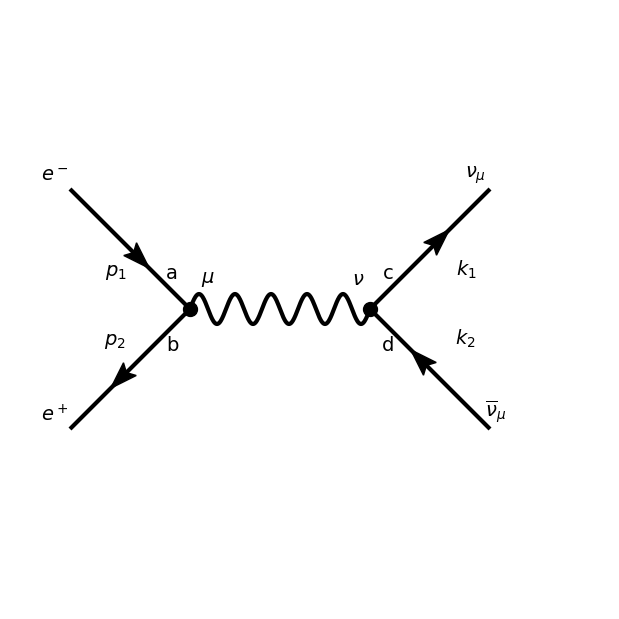
\includegraphics[width=0.7\linewidth]{13_6_feynman_diagram.png}
    \caption{Feynman diagram for $e^+e^-\rightarrow \overline{\nu}_\mu \nu_\mu$}
\end{figure}

\newpage

Before we find the cross section for this process, we need to determine the flux factor and Lorentz invariant phase space. We have the equation for the cross section:
\begin{align*}
    d\sigma=\frac{1}{(2E_1)(2E_2)|\vec{v}_1-\vec{v}_2|}|\mathcal{M}|^2d\Pi_{\text{LIPS}}
\end{align*}

However, we have done this calculation many times throughout the semester so I will just list the final result, as stated in Schwarz 13.69.
\begin{align*}
    \left(\frac{d\sigma}{d\Omega}\right)_\text{CM}=\frac{1}{64\pi^2E_\text{CM}^2}\frac{|\vec{p}_f|}{|\vec{p}_i|}|\mathcal{M}|^2
\end{align*}

Now we can start to calculate the matrix element. I will use equation 13.51 as a guide but replace the vertex and propagator as necessary. We will also take $m_Z^2\gg s$.
\begin{align*}
    i\mathcal{M}&=i\overline{v}(p_2)(g_V-g_A\gamma_5)\gamma^\mu u(p_1)\frac{-ig_{\mu\nu}}{k^2-m_Z^2+i\epsilon}i\overline{u}(p_3)(g_V-g_A\gamma_5)\gamma^\nu v(p_4) \\
    &= \frac{i}{-m_Z^2}\overline{v}(p_2)(g_V-g_A\gamma_5)\gamma^\mu u(p_1)\overline{u}(p_3)(g_V-g_A\gamma_5)\gamma_\mu v(p_4)
\end{align*}

There are 4 terms here, so when we square this, we are going to get 16 terms. To aid in solving this, I will write out the terms individually. Let's label each term by $T$.
\begin{align*}
    T_1&=-\frac{ig_V^2}{m_Z^2}\overline{v}(p_2)\gamma^\mu u(p_1)\overline{u}(p_3)\gamma_\mu v(p_4) \\
    T_2 &= \frac{ig_Vg_A}{m_Z^2}\overline{v} (p_2)\gamma^\mu u(p_1)\overline{u} (p_3)\gamma_5\gamma_\mu v(p_4) \\
    T_3 &= \frac{ig_Vg_A}{m_Z^2}\overline{v}(p_2)\gamma_5\gamma^\mu u(p_1)\overline{u}(p_3)\gamma_\mu v(p_4) \\
    T_4 &= -\frac{i g_A^2}{m_Z^2}\overline{v}(p_2)\gamma_5\gamma^\mu u(p_1)\overline{u}(p_3)\gamma_5\gamma_\mu v(p_4)
\end{align*}

We already solved the case $T_1T_1^\dagger$ and $T_4T_4^\dagger$ in the last problem, so we can cite those solutions. But, other than that, I'm not seeing a clever way to simplify our work if one exists. Thus, I am going to have to brute force all 16 terms. One nice thing is that we can ignore the masses. Let's go one by one. I will use the shorthand $u(p_1)\equiv u_1$ and same for $v$.

Before I start, though, I am going to go through one calcualtion that we will be doing over and over.
\begin{align*}
    \text{Tr}[\slashed{p}_1\gamma^\mu\slashed{p}_2\gamma^\nu] &=4p_{2\alpha}p_{1\beta}(g^{\alpha\mu}g^{\beta\nu}-g^{\alpha\beta}g^{\mu\nu}+g^{\alpha\nu}g^{\mu\beta}) \\ 
    &=4(p_2^\mu p_1^\nu-(p_2\cdot p_1) g_{\mu\nu}+p_2^\mu p_1^\nu) \\
    \text{Tr}[\slashed{p}_1\gamma_5\gamma^\mu\slashed{p}_2\gamma^\nu] &=4ip_{1\alpha}p_{2\beta}\epsilon^{\alpha \mu \beta \nu} \\ 
\end{align*}

With this knowledge, let's look at the first term.
\begin{align*}
    \sum_\text{spins}T_1T_1^\dagger&=\sum_\text{spins}\frac{g_V^4}{m_Z^4}(\overline{v}_2)_a (\gamma^\mu)_{ab}(u_1)_b (\overline{u}_3)_c (\gamma_\mu)_{cd} (v_4)_d (\overline{u}_1)_e (\gamma^\nu)_{ef}(v_2)_f (\overline{v}_4)_g (\gamma_\nu)_{gh} (u_3)_h \\
    &= \sum_\text{spins}\frac{g_V^4}{m_Z^4} (v_2)_f (\overline{v}_2)_a (\gamma^\mu)_{ab} (u_1)_b (\overline{u}_1)_e (\gamma^\nu)_{ef} (v_4)_d(\overline{v}_4)_g(\gamma_\nu)_{gh}(u_3)_h(\overline{u}_3)_c (\gamma_\mu)_{cd} \\
    &= \frac{g_V^4}{m_Z^4}\text{Tr}[\slashed{p}_2\gamma^\mu \slashed{p}_1 \gamma^\nu]\text{Tr}[\slashed{p}_4\gamma_\nu \slashed{p}_3 \gamma_\mu] \\
    &= \frac{16g_V^4}{m_Z^4} (p_1^\mu p_2^\nu + p_1^\nu p_2^\mu - g^{\mu\nu}(p_1\cdot p_2))(p_{3\mu} p_{4\nu} + p_{3\nu} p_{4\mu} - g_{\mu\nu}(p_3\cdot p_4)) \\
    &= \frac{32g_V^4}{m_Z^4}[(p_1\cdot p_3)(p_2 \cdot p_4)+(p_1\cdot p_4)(p_2\cdot p_3)] \\
    &= \frac{8g_V^4}{m_Z^4}(t^2+u^2)
\end{align*}

Honestly, that term alone took so much time that I don't know how I will finish all 16. But yet we continue on.
\begin{align*}
    \sum_\text{spins}T_1T_2^\dagger&=-\sum_\text{spins}\frac{g_V^3g_A}{m_Z^4}(\overline{v}_2)_a (\gamma^\mu)_{ab}(u_1)_b (\overline{u}_3)_c (\gamma_\mu)_{cd} (v_4)_d (\overline{u}_1)_e (\gamma^\nu)_{ef}(v_2)_f (\overline{v}_4)_g (\gamma_5\gamma_\nu)_{gh} (u_3)_h \\
    &=-\sum_\text{spins}\frac{g_V^3g_A}{m_Z^4}(v_2)_f(\overline{v}_2)_a (\gamma^\mu)_{ab}(u_1)_b(\overline{u}_1)_e (\gamma^\nu)_{ef}(v_4)_d(\overline{v}_4)_g (\gamma_5\gamma_\nu)_{gh} (u_3)_h(\overline{u}_3)_c (\gamma_\mu)_{cd}\\
    &= -\frac{g_V^3g_A}{m_Z^4}\text{Tr}[\slashed{p}_2\gamma^\mu \slashed{p}_1\gamma^\nu][\slashed{p}_4\gamma_5\gamma_\nu \slashed{p}_3\gamma_\mu] \\
    &=-\frac{16ig_V^3g_A}{m_Z^4}(p_1^\mu p_2^\nu + p_1^\nu p_2^\mu - g^{\mu\nu}(p_1\cdot p_2))(p_4^\alpha p_3^\beta \epsilon_{\alpha \nu \beta \mu})
\end{align*}

Here we see something nice: the first trace is symmetric about $\mu\leftrightarrow \nu$, while the second trace is anti-symmetric. Thus, summing over $\mu$ and $\nu$ will cancel everything out - we get 0!
\begin{align*}
    \sum_\text{spins}T_1T_2^\dagger&=0
\end{align*}

This is a huge simplification: any trace without $\gamma_5$ is symmetric under exchange of $\mu$ and $\nu$, and any trace with $\gamma_5$ is anti-symmetric. Thus, all the terms with an odd number of $\gamma_5$ traces will all be 0. This reduces the number of terms we need to look at. We see that $T_1$ and $T_4$ have an even number of $\gamma_5$ matrices, while $T_2$ and $T_3$ have an odd number. So, any cross term involving these two sets will be 0. Thus, we only need to look at a few number of terms.
\begin{align*}
    (T_1T_1^\dagger, T_1T_4^\dagger, T_4T_1^\dagger, T_4T_4^\dagger), (T_2T_2^\dagger, T_2T_3^\dagger, T_3T_2^\dagger, T_3T_3^\dagger)
\end{align*}

And we forge ahead, now looking at our next non-zero term.
\begin{align*}
    \sum_\text{spins}T_1T_4^\dagger&=\sum_\text{spins}\frac{g_V^2g_A^2}{m_Z^4}(\overline{v}_2)_a (\gamma^\mu)_{ab}(u_1)_b (\overline{u}_3)_c (\gamma_\mu)_{cd} (v_4)_d (\overline{u}_1)_e (\gamma_5\gamma^\nu)_{ef}(v_2)_f (\overline{v}_4)_g (\gamma_5\gamma_\nu)_{gh} (u_3)_h \\
    &= \sum_\text{spins}\frac{g_V^2g_A^2}{m_Z^4}(v_2)_f(\overline{v}_2)_a (\gamma^\mu)_{ab}(u_1)_b(\overline{u}_1)_e (\gamma_5\gamma^\nu)_{ef}(v_4)_d(\overline{v}_4)_g (\gamma_5\gamma_\nu)_{gh} (u_3)_h(\overline{u}_3)_c (\gamma_\mu)_{cd} \\
    &= \frac{g_V^2g_A^2}{m_Z^4}\text{Tr}[\slashed{p}_2\gamma^\mu\slashed{p}_1\gamma_5\gamma^\nu]\text{Tr}[\slashed{p}_4\gamma_5\gamma_\nu\slashed{p}_3\gamma_\mu] \\
    &= -\frac{16g_V^2g_A^2}{m_Z^4}p_{2\alpha}p_{1\beta}p_4^\rho p_3^\sigma \epsilon^{\alpha\mu\beta\nu}\epsilon_{\rho\nu\sigma\mu}
\end{align*}

Now we will use the identity $\epsilon^{\alpha\beta\mu\nu}\epsilon_{\rho\sigma\mu\nu}=2(\delta^\alpha_\rho\delta^\beta_\sigma-\delta^\alpha_\sigma\delta^\beta_\rho)$. See [1] for a discussion on this. To get our $\epsilon$ tensors in this form, we need to swap 3 indices: 1 in the first tensor in 2 in the second. So, we pick up a negative sign.
\begin{align*}
    \sum_\text{spins}T_1T_4^\dagger&=\frac{16g_V^2g_A^2}{m_Z^4}(p_2\cdot p_4)(p_1 \cdot p_3)-(p_2\cdot p_3)(p_1 \cdot p_4) \\
    &= \frac{4g_V^2g_A^2}{m_Z^4}(t^2-u^2)
\end{align*}

Let's now look at $T_4T_1^\dagger$ just in case they end up cancelling and we can simplify our work even more.
\begin{align*}
    \sum_\text{spins}T_4T_1^\dagger&=\sum_\text{spins}\frac{g_V^2g_A^2}{m_Z^4}(\overline{v}_2)_a (\gamma_5\gamma^\mu)_{ab}(u_1)_b (\overline{u}_3)_c (\gamma_5\gamma_\mu)_{cd} (v_4)_d (\overline{u}_1)_e (\gamma^\nu)_{ef}(v_2)_f (\overline{v}_4)_g (\gamma_\nu)_{gh} (u_3)_h \\
    &= \sum_\text{spins}\frac{g_V^2g_A^2}{m_Z^4}(v_2)_f(\overline{v}_2)_a (\gamma_5\gamma^\mu)_{ab}(u_1)_b(\overline{u}_1)_e (\gamma^\nu)_{ef}(v_4)_d(\overline{v}_4)_g (\gamma_\nu)_{gh} (u_3)_h(\overline{u}_3)_c (\gamma_5\gamma_\mu)_{cd} \\
    &=\frac{g_V^2g_A^2}{m_Z^4}\text{Tr}[\slashed{p}_2\gamma_5\gamma^\mu\slashed{p}_1\gamma^\nu]\text{Tr}[\slashed{p}_4\gamma_\nu\slashed{p}_3\gamma_5\gamma_\mu] \\
    &= -\frac{16g_V^2g_A^2}{m_Z^4}p_{2\alpha}p_{1\beta}p_4^\rho p_3^\sigma \epsilon^{\alpha\mu\beta\nu}\epsilon_{\rho\nu\sigma\mu} \\
    &= \frac{16g_V^2g_A^2}{m_Z^4}(p_2\cdot p_4)(p_1 \cdot p_3)-(p_2\cdot p_3)(p_1 \cdot p_4) \\
    &= \frac{4g_V^2g_A^2}{m_Z^4}(t^2-u^2)
\end{align*}

So we see that they are equal. This simplifies our work more: we will say that the cross terms are all equal. Note that I haven't necessarily proved that, but let's just guess it is the case so we can save on some time. Our last term in this group is $T_4T_4^\dagger$.
\begin{align*}
    \sum_\text{spins}T_4T_4^\dagger&=\sum_\text{spins}\frac{g_A^4}{m_Z^4}(\overline{v}_2)_a (\gamma_5\gamma^\mu)_{ab}(u_1)_b (\overline{u}_3)_c (\gamma_5\gamma_\mu)_{cd} (v_4)_d (\overline{u}_1)_e (\gamma_5\gamma^\nu)_{ef}(v_2)_f (\overline{v}_4)_g (\gamma_5\gamma_\nu)_{gh} (u_3)_h \\
    &= \sum_\text{spins}\frac{g_A^4}{m_Z^4}(v_2)_f(\overline{v}_2)_a (\gamma_5\gamma^\mu)_{ab}(u_1)_b(\overline{u}_1)_e (\gamma_5\gamma^\nu)_{ef}(v_4)_d(\overline{v}_4)_g (\gamma_5\gamma_\nu)_{gh} (u_3)_h(\overline{u}_3)_c (\gamma_5\gamma_\mu)_{cd}\\
    &=\frac{g_A^4}{m_Z^4}\text{Tr}[\slashed{p}_2\gamma_5\gamma^\mu\slashed{p}_1\gamma_5\gamma^\nu]\text{Tr}[\slashed{p}_4\gamma_5\gamma_\nu\slashed{p}_3\gamma_5\gamma_\mu] \\
    &= \frac{g_A^4}{m_Z^4}\text{Tr}[\slashed{p}_2\gamma^\mu\slashed{p}_1\gamma^\nu]\text{Tr}[\slashed{p}_4\gamma_\nu\slashed{p}_3\gamma_\mu]
\end{align*}

Thus, we see that $T_4T_4^\dagger$ is the same as $T_1T_1^\dagger$ if we swap $g_V\rightarrow g_A$. We have now done all the terms with an even number of $\gamma_5$ matrices.
\begin{align*}
    \text{Even number of $\gamma_5$: }\sum_\text{spins}|\mathcal{M}|^2=\frac{8}{m_Z^4}(g_V^4+g_A^4)(t^2+u^2)+\frac{8g_V^2g_A^2}{m_Z^4}(t^2-u^2)
\end{align*} 

Now we go to look at all the terms with an odd number of $\gamma_5$ matrices. Let's start with $T_2T_2^\dagger$. We eventually get to an expression that we solved before when looking at $T_1T_1^\dagger$, so I will skip some steps.
\begin{align*}
    \sum_\text{spins}T_2T_2^\dagger&=\sum_\text{spins}\frac{g_V^2g_A^2}{m_Z^4}(\overline{v}_2)_a (\gamma^\mu)_{ab}(u_1)_b (\overline{u}_3)_c (\gamma_5\gamma_\mu)_{cd} (v_4)_d (\overline{u}_1)_e (\gamma^\nu)_{ef}(v_2)_f (\overline{v}_4)_g (\gamma_5\gamma_\nu)_{gh} (u_3)_h \\
    &=\sum_\text{spins}\frac{g_V^2g_A^2}{m_Z^4}(v_2)_f(\overline{v}_2)_a (\gamma^\mu)_{ab}(u_1)_b(\overline{u}_1)_e (\gamma^\nu)_{ef}(v_4)_d(\overline{v}_4)_g (\gamma_5\gamma_\nu)_{gh} (u_3)_h(\overline{u}_3)_c (\gamma_5\gamma_\mu)_{cd} \\
    &=\frac{g_V^2g_A^2}{m_Z^4}\text{Tr}[\slashed{p}_2\gamma^\mu\slashed{p}_1\gamma^\nu]\text{Tr}[\slashed{p}_4\gamma_5\gamma_\nu\slashed{p}_3\gamma_5\gamma_\mu] \\
    &= \frac{g_V^2g_A^2}{m_Z^4}\text{Tr}[\slashed{p}_2\gamma^\mu\slashed{p}_1\gamma^\nu]\text{Tr}[\slashed{p}_4\gamma_\nu\slashed{p}_3\gamma_\mu] \\
    &= \frac{8g_V^2g_A^2}{m_Z^4}(t^2+u^2)
\end{align*}

We expect to get the same thing from $T_3T_3^\dagger$. The last thing we need to check is the cross terms. We see, again, the same pattern from the cross terms in the other calculations we just did.
\begin{align*}
    \sum_\text{spins}T_2T_3^\dagger&=\sum_\text{spins}\frac{g_V^2g_A^2}{m_Z^4}(\overline{v}_2)_a (\gamma^\mu)_{ab}(u_1)_b (\overline{u}_3)_c (\gamma_5\gamma_\mu)_{cd} (v_4)_d (\overline{u}_1)_e (\gamma_5\gamma^\nu)_{ef}(v_2)_f (\overline{v}_4)_g (\gamma_\nu)_{gh} (u_3)_h \\
    &= \sum_\text{spins}\frac{g_V^2g_A^2}{m_Z^4}(v_2)_f(\overline{v}_2)_a (\gamma^\mu)_{ab}(u_1)_b(\overline{u}_1)_e (\gamma_5\gamma^\nu)_{ef}(v_4)_d(\overline{v}_4)_g (\gamma_\nu)_{gh} (u_3)_h(\overline{u}_3)_c (\gamma_5\gamma_\mu)_{cd} \\
    &= \frac{g_V^2g_A^2}{m_Z^4}\text{Tr}[\slashed{p}_2\gamma^\mu\slashed{p}_1\gamma_5\gamma^\nu]\text{Tr}[\slashed{p}_4\gamma_\nu\slashed{p}_3\gamma_5\gamma_\mu] \\
    &= \frac{4g_V^2g_A^2}{m_Z^4}(t^2-u^2)
\end{align*}

We expect the same thing from $T_3T_2^\dagger$. So, we can get the sum of all the terms with an odd number of $\gamma_5$ matrices.
\begin{align*}
    \text{Odd number of $\gamma_5$: }\sum_\text{spins}|\mathcal{M}|^2&=\frac{16g_V^2g_A^2}{m_Z^4}(t^2+u^2)+\frac{8g_V^2g_A^2}{m_Z^4}(t^2-u^2) \\
    &=\frac{8g_V^2g_A^2}{m_Z^4}(3t^2+u^2)
\end{align*} 

So, now we put it all together. But since we are averaging over incoming spin, we need to divide by 4.:
\begin{align*}
    \text{Total: }\frac{1}{4}\sum_\text{spins}|\mathcal{M}|^2&=\frac{2}{m_Z^4}(g_V^4+g_A^4)(t^2+u^2)+\frac{2g_V^2g_A^2}{m_Z^4}(t^2-u^2)+\frac{2g_V^2g_A^2}{m_Z^4}(3t^2+u^2) \\
    &= \frac{2}{m_Z^4}(g_V^4+g_A^4)(t^2+u^2)+\frac{8g_V^2g_A^2}{m_Z^4}t^2
\end{align*}

Now we plug this into our expression for the differential cross section. Following the notation of equation 13.73 in the book:
\begin{align*}
    \frac{d\sigma}{d\Omega}&=\frac{1}{64\pi^2E_\text{CM}^2}\frac{|\vec{p}_f|}{|\vec{p}_i|}\|\mathcal{M}|^2 \\
    &=\frac{1}{32\pi^2 E_\text{CM}^2m_Z^4}\frac{|\vec{p}|}{|\vec{k}|}\left[(g_V^4+g_A^4)(t^2+u^2)+4g_V^2g_A^2t^2\right]
\end{align*}

We make the substitution $t=-2E^2+2\vec{k}\cdot\vec{p}$ and $u=-2E^2-2\vec{k}\cdot\vec{p}$, where $E_\text{CM}^2=4E^2$. Again, this is all outlined in equation 13.73.
\begin{align*}
    \frac{d\sigma}{d\Omega}&=\frac{1}{32\pi^2 E_\text{CM}^2m_Z^4}\frac{|\vec{p}|}{|\vec{k}|}\left(8(g_V^4+g_A^4)(E^4+(\vec{k}\cdot\vec{p})^2)+4g_V^2g_A^2(4E^4-8E^2\vec{k}\cdot\vec{p}+4(\vec{k}\cdot\vec{p})^2)\right) \\
    &= \frac{1}{8\pi^2 E_\text{CM}^2m_Z^4}\left((g_V^4+g_A^4)(E^4+(\vec{k}\cdot\vec{p})^2)+2g_V^2g_A^2(E^4-2E^2\vec{k}\cdot\vec{p}+(\vec{k}\cdot\vec{p})^2)\right)
\end{align*}

Now we use $\vec{k}\cdot\vec{p}=|\vec{k}||\vec{p}|\cos\theta$ to add in angular dependence. Additionally, $|\vec{k}|=|\vec{p}|=E$ since we are ignoring the particle masses and working in the COM frame.
\begin{align*}
    \frac{d\sigma}{d\Omega}&=\frac{1}{32\pi^2 E^2m_Z^4}\left((g_V^4+g_A^4)E^4(1+\cos^2\theta)+2E^4g_V^2g_A^2(1-2\cos\theta+\cos^2\theta)\right) \\
    &= \frac{E^2}{32\pi^2 m_Z^4}\left((g_V^4+g_A^4)(1+\cos^2\theta)+2g_V^2g_A^2(1-\cos\theta)^2\right) \\
    &= \frac{E_\text{CM}^2}{8\pi^2 m_Z^4}\left((g_V^4+g_A^4)(1+\cos^2\theta)+2g_V^2g_A^2(1-\cos\theta)^2\right)
\end{align*}

Do I think this is correct? Probably not, though I believe I did the correct steps. It is likely I made a mathematical mistake somewhere. Even so, let's just claim this is the result.
\begin{align*}
    \boxed{\frac{d\sigma}{d\Omega}=\frac{E_\text{CM}^2}{8\pi^2 m_Z^4}\left((g_V^4+g_A^4)(1+\cos^2\theta)+2g_V^2g_A^2(1-\cos\theta)^2\right)}
\end{align*}

\end{solution}

\begin{questionpart}{c}
Find values of $g_V$ and $g_A$ that reproduce the picture in the book. Show that this choice is equivalient to the Z boson have chiral couplings only to the left-handed fields. Argue this is evidence of parity violation.
\end{questionpart}

We want to tune $g_V$ and $g_A$ so that our cross section approaches 0 as $\cos\theta$ approaches 1. Unfortunately, I cannot get a graph that looks like this.

However, based on the question I can propose that the correct answer should be $g_V=g_A$. This means that our vertex Feynman rule takes the form $ig(1-\gamma_5)\gamma^\mu$. And we recognize $1-\gamma_5$ as being the left-chiral projection operator $P_L=\frac{1-\gamma_5}{2}$. Thus, the vertex will only interact with left-handed fields, as the projection operator will give us 0 for right-handed fields.
This violates parity because the process would not be the same under a parity transformation, as the fields would change but the coupling wouldn't.

\newpage
[1] https://math.stackexchange.com/questions/4544165/how-to-contract-a-4th-rank-levi-civita-tensor

\end{document}
